\documentclass{article}
\usepackage[utf8]{inputenc}
\usepackage{graphicx}
\usepackage{listings}
\usepackage{xcolor}

\colorlet{punct}{red!60!black}
\definecolor{background}{HTML}{EEEEEE}
\definecolor{delim}{RGB}{20,105,176}
\colorlet{numb}{magenta!60!black}

\lstdefinelanguage{json}{
    basicstyle=\normalfont\ttfamily,
    numbers=left,
    numberstyle=\scriptsize,
    stepnumber=1,
    numbersep=8pt,
    showstringspaces=false,
    breaklines=true,
    frame=lines,
    backgroundcolor=\color{background},
    literate=
     *{0}{{{\color{numb}0}}}{1}
      {1}{{{\color{numb}1}}}{1}
      {2}{{{\color{numb}2}}}{1}
      {3}{{{\color{numb}3}}}{1}
      {4}{{{\color{numb}4}}}{1}
      {5}{{{\color{numb}5}}}{1}
      {6}{{{\color{numb}6}}}{1}
      {7}{{{\color{numb}7}}}{1}
      {8}{{{\color{numb}8}}}{1}
      {9}{{{\color{numb}9}}}{1}
      {:}{{{\color{punct}{:}}}}{1}
      {,}{{{\color{punct}{,}}}}{1}
      {\{}{{{\color{delim}{\{}}}}{1}
      {\}}{{{\color{delim}{\}}}}}{1}
      {[}{{{\color{delim}{[}}}}{1}
      {]}{{{\color{delim}{]}}}}{1},
}
\title{Relazione Hanabi}
\author{Mihail Bida, Francesco Pandolfi }
\date{December 2020}

\begin{document}

\maketitle

\section{Introduzione}
\subsection{Regolamento}
\begin{itemize}
    \item Il mazzo di Hanabi è formato da 50 carte suddivise in 5 colori (10 per ogni colore). Ogni colore è composto: 3 carte di valore 1, 2 di valore 2,3,4 e 1 di valore 5.
    \item In campo ci sono 8 gettoni informazione e 3 gettoni errore
    \item Ogni giocatore tiene le proprie carte rivolte verso gli altri (4 carte in 4 o 5 giocatori e 5 carte in 2 o 3 giocatori), quindi vede tutto tranne le proprie carte.
    \item Lo scopo del gioco è completare le scale di colore da 1 a 5. Ogni carta giocata vale 1 punto.
    \item 
    {Ad ogni turno ogni giocatore può fare una delle seguenti mosse:
    \begin{itemize}
        \item indicare ad un giocatore tutte le carte di uno stesso colore o valore nella sua mano.
        \item scartare una carta dalla propria mano.
        \item giocare una carta.
    \end{itemize}}
    \item Giocare o scartare una carta fa pescare una carta dal mazzo. Finite le carte da pescare, il gioco termina quando è nuovamente il turno di chi ha pescato l’ultima carta.
    \item Scartare una carta aumenta i gettoni informazione di 1 (fino ad un massimo di 8).
    \item Giocare una carta sbagliata fa perdere un gettone errore. Finiti i gettoni errore la partita è conclusa con punteggio 0.
\end{itemize}

\subsection{Stato dell'arte}
Negli ultimi anni è stata prodotta un'ampia varietà di agenti. Come riporta il paper The Hanabi Challenge: A New Frontier for AI Research\footnote{ https://arxiv.org/pdf/1902.00506.pdf} hanabi ha destato l'interesse dei ricercatori in quanto gioco cooperativo, che quindi permette di studiare soluzioni di intelligenza artificiale in uno scenario molto diverso da quello offerto dai giochi competitivi.
Tuttavia si è notato che gli agenti intelligenti sono surclassati da agenti che eseguono strategie codificate dal programmatore.\newline
\newline
La strategia proposta dagli autori del paper è incentrata sulla comunicazione implicita, ossia lo stabilire un insieme di convenzioni che permettano di aggiungere informazioni quando si dà un suggerimento. Ciò è necessario in quanto il numero di suggerimenti che si possono dare in una partita è limitato.

\section{Strategia adottata}
\begin{flushleft}
Le strategie di gioco presentate durante il corso di Fondamenti di Intelligenza Artificiale M consistono in varianti di ricerca nello spazio degli stati.\newline
Abbiamo poi visto come l'algoritmo min-max sia molto efficace nei giochi competitivi e come sia possibile attraverso pruning diminuire considerevolmente il numero di stati che è necessario esplorare.\newline
Nostro malgrado Hanabi è un gioco cooperativo e questo ci preclude la possibilità di sfruttare sia min-max sia il pruning. \newline
\newline
Lo spazio degli stati di una partita di Hanabi è molto vasto, sebbene solo le giocate e le scartate generino complessità. Quando si dà un suggerimento esiste un solo  stato possibile, ma se si gioca o scarta una carta non si sa sempre con certezza quale carta si sta giocando o scartando. Inoltre si deve pescare dal mazzo, il che dà incertezza sulla carta pescata. \newline
La tabella 1 mostra un'approssimazione del numero di stati da esplorare per conoscere completamente tutti i possibili stati che si possono raggiungere con giocate o scartate a partire da uno stato dato.
\end{flushleft}
\begin{table}[h]
    \centering
    \begin{tabular}{m|s}
        \toprule
        \textbf{Numero di giocatori} & \textbf{Numero di stati} \\
        \midrule
        2 & [10(m)(c)+10)^d \\
        3 & [10(m)(c)+20]^d \\
        4 & [8(m)(c)+12]^d \\
        5 & [8(m)(c)+16]^d \\
    \end{tabular}
    \caption{Cardinalità spazio degli stati in funzione del numero di giocatori}
\end{table}

\begin{flushleft}
La dimensione dello spazio degli stati varia in modo esponenziale in funzione della profondità di esplorazione richiesta (d), come i giochi tradizionali, stile scacchi, ma in più l'incertezza sulle proprie carte e su quelle pescate fa crescere il numero di stati secondo una funzione polinomiale di due fattori: il numero di carte rimaste nel mazzo (m) e il numero di carte che quella che si vuole giocare/scartare potrebbe essere (c).\newline
\newline

Hanabi possiede uno spazio degli stati più vasto anche degli altri giochi di carte, per lo più competitivi, in cui si conosce la propria mano ma non quelle degli altri giocatori. In questi casi infatti non si ha la componente di incertezza dovuta al non conoscere le proprie carte.
\newline
\newline
Le strategie seguite dai bot prodotti consistono nel valutare se fare un tipo di mossa in funzione di 3 parametri calcolati per le carte coinvolte dalla mossa:
\begin{itemize}
    \item entropia: incertezza sul tipo di carta. Se la carta è completamente conosciuta la sua entropia è 0. Abbiamo notato empiricamente che una mano completamente sconosciuta ha un'entropia di circa 22 bit (dipende dal numero di carte in mano e dal numero di giocatori).
    
    \item giocabilità: probabilità che giocando una carta non si commetta errore 
    
    \item inutilità: probabilità che scartando una carta non si comprometta il punteggio finale.
\end{itemize}
Giocare una carta sarà una buona mossa se la giocabilità di quella carta è alta, situazione analoga per lo scartare una carta con alta inutilità. Un buon consiglio invece cercherà di alzare la giocabilità delle carte del compagno. Il parametro di entropia viene per lo più usato per selezionare il miglior consiglio nei casi in cui più consigli fanno raggiungere ad una carta lo stesso valore di giocabilità o inutilità.\newline
\newline
In generale, l'effetto di una mossa, inteso come variazione dei parametri che descrivono lo stato attuale, è visibile solo tra lo stato attuale e quello generato. Negli stati successivi al generato la mossa non produrrà altre variazioni.\newline
Per questo motivo riteniamo che un'esplorazione profonda non aggiunga informazioni rilevanti che aiutino a prendere una decisione sulla mossa da effettuare rispetto alla sola esplorazione degli stati più prossimi a quello attuale. \newline
\newline
Ad esempio, si prenda una partita tra 3 giocatori: A,B e C.\newline
C sa che ha in mano un tre giallo, ma la scala gialla è a uno, quindi vede una giocabilità sul tre giallo pari a 0.\newline B sa che una sua carta è gialla.\newline A vede che la carta che B sa essere gialla è un due, quindi decide di suggerirgli i due.\newline B gioca il due giallo.\newline Ora C vede una giocabilità pari a 1 e gioca il tre.\newline
\newline

Il suggerimento di A verso B rende possibile la giocata di due carte dando informazioni solo a B. Durante la transizione tra il turno in cui tocca a B e il turno in cui tocca a C, il suggerimento di A non gioca alcun ruolo. C ottiene l'informazione che modifica la giocabilità del tre giallo dalla giocata di B.\newline
Ogni mossa propaga informazioni solo allo stato generato. \newline
\newline

Giocabilità e inutilità di una data carta sono calcolate sommando per ogni tipo di carta giocabile/inutile le probabilità che la carta data sia proprio di quel tipo. \newline
Sebbene la definizione di carta giocabile sia semplice (una carta è giocabile se la scala del suo colore ha valore precedente a quello della carta data), altrettanto non vale per la definizione di carta inutile. Una carta è inutile se è vera almeno una delle seguenti condizioni:
\begin{itemize}
    \item La scala dello stesso colore ha valore maggiore o uguale della carta.\newline
    Se ad esempio la scala rossa termina con un 4, tutte le carte rosse tranne il 5 sono inutili.
    \item Tra gli scarti sono presenti tutti gli esemplari di carte di stesso colore e uno qualsiasi dei valori inferiori.\newline
    Ad esempio i 3, i 4 e il 5 rosso sono inutili se tutti i 2 rossi sono stati scartati.
    \item Almeno una copia della carta è nel mazzo o in mano ad un compagno.\newline
    Se ad esempio 2 copie di una carta inutile sono in mano ai giocatori vengono viste entrambe come inutili. Quando una delle due viene scartata l'altra non sarà più inutile.
\end{itemize}
\end{flushleft}
L'entropia invece è calcolata secondo la formula classica.


\section{Bot prodotti}
Abbiamo sviluppato due bot, Bot1 e Bot2 che seguono due strategie differenti ma con alcuni punti in comune. Il più importante di questi è che durante la valutazione di una mossa il bot si immedesima negli altri giocatori e valuta calcolando i parametri dal loro punto di vista, introducendo un errore sistematico nelle valutazioni: un giocatore che si immedesima in un altro non conosce le proprie carte, mentre gli altri le vedono. Questo è un motivo in più per rinunciare ad un'esplorazione profonda dello spazio degli stati.\newline
\newline
La strategia di Bot1 potrebbe essere definita "altruista": all'inizio del suo turno il bot osserva la situazione dei suoi compagni e li classifica in fasi:
\begin{itemize}
    \item Fase 1: il compagno ha una carta con giocabilità 1 (quindi può giocare sicuro).
    \item Fase 2: il compagno ha una carta con inutilità 1 (quindi può scartare sicuro).
    \item Fase 3: il numero di gettoni rimasti è maggiore del numero di turni che devono passare affinché tocchi al giocatore (quindi il compagno potrà sicuramente suggerire)
    \item Fase 4 (o critica): nessuna delle condizioni precedenti è soddisfatta (il giocatore non può suggerire e qualsiasi mossa faccia rischia di sbagliare)
\end{itemize}
Se Bot1 ha compagni in fase critica cercherà il miglior suggerimento da dare al primo di loro (in ordine di gioco) in modo che raggiunga la fase di indice più basso possibile. In caso di parità darà il suggerimento che abbassa di più l'entropia della mano.\newline
Se nessuno dei compagni di Bot1 è in fase critica il bot cercherà di compiere la prima azione possibile di questa lista:
\begin{enumerate}
    \item gioca una carta sicura.
    \item se i gettoni suggerimento sono superiori ad un certo limite (numero di giocatori) allora dà il miglior suggerimento al giocatore in fase peggiore (in caso di parità si suggerisce al giocatore cui tocca prima).
    \item scarta la carta con inutilità più alta.
\end{enumerate}

\begin{flushleft}
Bot2 è stato pensato per implementare una strategia più aggressiva: si tende a giocare immediatamente le carte sicure e a suggerire in modo da aumentare la giocabilità delle carte che possono essere giocate. Le mosse scelte inoltre tendono ad aumentare il numero di carte giocabili tra quelle possedute dai giocatori. Come prima, il bot cercherà di effettuare la prima azione possibile della seguente lista:
\begin{enumerate}
    \item  gioca una carta sicura. Nel caso in cui avesse più carte giocabili gioca quella che rende giocabili il maggior numero di carte possedute dai giocatori.
    \item se ha gettoni suggerimento, controlla gli altri giocatori: se uno ha una carta giocabile non sicura gli dà il suggerimento più significativo (in termini di diminuzione dell'entropia della mano) che coinvolge quella carta. Nel caso in cui il giocatore avesse più carte giocabili non sicure gli indica quella che, se giocata, rende giocabili il maggior numero di carte possedute dai giocatori.
    Questo consiglio viene dato solo se la carta è resa sicuramente giocabile.
    \item se non c'è un gettone suggerimento per giocatore e ha una carta sicura da scartare la scarta.
  \item se ha almeno un gettone suggerimento prova a suggerire come nel punto 2 anche se la carta non è resa sicuramente giocabile.
  \item se ha almeno un gettone suggerimento dà il suggerimento (a qualsiasi giocatore) che diminuisce del massimo l'entropia delle carte.
    \item scarta la carta con uselessness maggiore.
\end{enumerate}
Segue la tabella che mostra i risultati raggiunti dai bot calcolati su 100 partite con numero di giocatori pari e 50 e 50, alternando il bot con più esemplari, per le partite con numero di giocatori dispari. In questi casi è mostrata la media dei punteggi medi e delle deviazioni, e i minimi e massimi assoluti (tra parentesi è indicato quale bot aveva più esemplari nel raggiungimento di quel punteggio).
\end{flushleft}
\begin{table}[h]
    \centering
    \begin{tabular}{m|b|b|b}
        \toprule
        \textbf{Numero di giocatori} & \textbf{Bot1} & \textbf{Bot2} & \textbf{Bot1/Bot2} \\
        \midrule
        2 & 11.77 2.88 17 6 & 14.37 3.07 20 8 & 12.71 2.90 19 8\\
        3 & \textbf{11.81} 2.48 17 6 & \textbf{17.65} 1.53 21 13& \textbf{15.14} 2.24 18(2) 8(2) \\
        4 & 8.86 2.15 14 2 & 17.25 1.31 20 14 & 13.35 2.17 19 7\\
        5 & 9.44 2.11 15 4 & 16.33 1.11 19 14 & 13.12 1.75 17(2) 8(1)  \\
    \end{tabular}
    \caption{Tabella che mostra i punteggi medi,  deviazione standard, massimo e minimo su 100 partite}
\end{table}


\section{Possibili sviluppi}
Bot1 e Bot2 non raggiungono punteggi elevati per motivi differenti: Bot1 tende a scartare molte più carte di quante ne gioca, arrivando quindi in fretta alla fine della partita. Bot2 invece perde punti perchè scarta tutti gli esemplari di carte che erano ancora da giocare.\newline
L'adozione di convenzioni dovrebbe permettere di superare questi limiti.\newline
\newline
Un esempio di convenzione che dovrebbe migliorare le prestazioni si basa sul fatto che non ci sono limitazioni su come ordinare le carte nella mano dei giocatori. La convenzione impone di posizionare l'ultima carta pescata nella posizione più a destra nella propria mano e di suggerire le carte giocabili o da non scartare dando la precedenza a quelle a destra. In questo modo si lasciano implicitamente le carte da scartare nella parte sinistra della mano.\newline
\newline
Un altro esempio può essere lo stabilire che se un giocatore riceve un suggerimento che coinvolge una sola carta deve giocarla.\newline
\newline
Dal punto di vista dell'implementazione degli agenti, le convenzioni hanno il costo di dover tenere traccia di tutti i suggerimenti, dati e ricevuti, e delle informazioni implicite che essi trasportano per convenzione. Inoltre è possibile che la ricerca della mossa migliore richieda un'esplorazione degli stati più profonda di quella effettuata dai bot presentati, a seconda di come la convenzione è formulata.

\section{Framework hanabi-unibo}
Il framework hanabi-unibo è stato prodotto ex novo come soluzione portabile ed estendibile. Scritto completamente in java è composto da più moduli:
\begin{itemize}
    \item hanabi-api: contiene classi di supporto agli altri moduli
    \item hanabi-game: eseguibile, implementa il server host della partita. 
    \item hanabi-human-player: eseguibile, offre una GUI di gioco per utente umano.
    \item hanabi-bot1: eseguibile, implementa Bot1.
    \item hanabi-bot2: eseguibile, implementa Bot2.
\end{itemize}
Tutti gli eseguibili offrono un'interfaccia grafica swing e possono essere avviati con doppio click. In alternativa, l'avvio da terminale permetterà di vedere il log di esecuzione.\newline
\newline
Per iniziare una partita si deve avviare l'host hanabi-game e impostare le configurazioni della partita.\newline
Una volta confermata la configurazione, l'host attenderà una connessione tcp alla porta indicata per ogni giocatore indicato come non chiuso. Se il giocatore non è indicato come aperto allora il programma avvierà automaticamente l'eseguibile indicato.\newline
\newline
Durante la partita i giocatori comunicano con l'host attraverso il seguente protocollo

\begin{figure}[h]
\centering
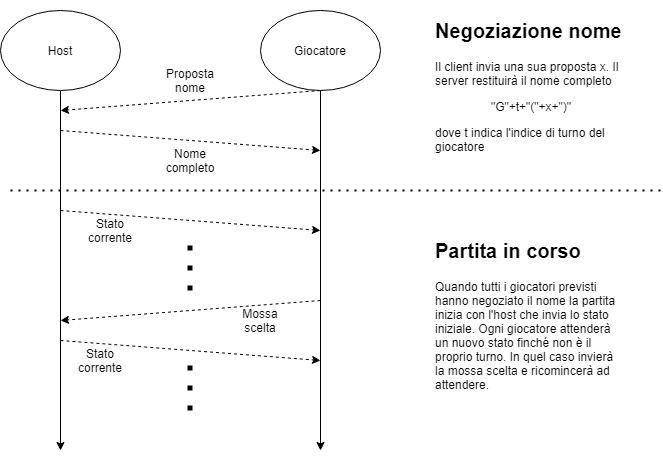
\includegraphics[width=0.9\textwidth]{Protocol.png}
\end{figure}
\begin{flushleft}
I nomi sono inviati come stringhe seguite da un carattere terminatore di riga, gli stati e le mosse invece sono modellati come oggetti json, alla pari degli altri concetti chiave del gioco, come le carte, le mani e le scale di colore.\newline
\newline
Segue un esempio di stato inviato dall'host a G2(Human). Rappresenta il secondo stato di una partita a due giocatori, tra un umano e un Bot1. Bot1 ha eseguito la prima mossa che è stata un suggerimento delle carte di valore 3.
\newline
\small
\begin{lstlisting}[language=json,firstnumber=1]
{
   "discarded":[],
   "green": 0,
   "hints": 7,
   "deck": 40,
   "yellow": 0,
   "red": 0,
   "fuse": 3,
   "current":"G2 (Human)",
   "white": 0,
   "blue": 0,
   "round": 2,
   "G2 (Human)":[
      {"color":null,"possible_values":[1,2,4,5],"value":0,"possible_colors":["red","green","white","blue","yellow"]},
      {"color":null,"possible_values":[3],"value":3,"possible_colors":["red","green","white","blue","yellow"]},
      {"color":null,"possible_values":[3],"value":3,"possible_colors":["red","green","white","blue","yellow"]},
      {"color":null,"possible_values":[1,2,4,5],"value":0,"possible_colors":["red","green","white","blue","yellow"]},
      {"color":null,"possible_values":[3],"value":3,"possible_colors":["red","green","white","blue","yellow"]}
    ],
   "final": -1,
   "G1 (Bot1)":[
      {"color":"white","possible_values":[1,2,4,5,3],"value":4,"possible_colors":["red","green","white","blue","yellow"]},
      {"color":"yellow","possible_values":[1,2,4,5,3],"value":1,"possible_colors":["red","green","white","blue","yellow"]},
      {"color":"green","possible_values":[1,2,4,5,3],"value":1,"possible_colors":["red","green","white","blue","yellow"]},
      {"color":"yellow","possible_values":[1,2,4,5,3],"value":2,"possible_colors":["red","green","white","blue","yellow"]},
      {"color":"red","possible_values":[1,2,4,5,3],"value":2,"possible_colors":["red","green","white","blue","yellow"]}
    ],
   "lastaction":{"hinted":"G2(Human)","type":"hintvalue","value":3,"player":"G1(Bot1)"}
}
\end{lstlisting}
\normalsize
Il campo final indica l'ultimo turno di gioco, o vale -1 se ancora ci sono carte nel mazzo. Il campo round indica il turno corrente. Quando il campo final ha valore uguale a quello di round si ha l'ultimo stato della partita. Man mano che i giocatori ricevono gli stati dall'host controllano questi due campi: se sono uguali smettono di seguire il protocollo di gioco e la partita finisce. \newline
\newline
Il modulo hanabi-api implementa i concetti chiave sfruttando la libreria di supporto json-v2. Inoltre implementa i componenti grafici e offre classi utili allo sviluppo di nuovi bot: GameClient, che implementa il protocollo di gioco, e Analitics, che offre metodi per l'analisi di uno stato della partita. I bot prodotti sono stati costruiti usando queste classi e i loro sorgenti costituiscono degli ottimi esempi d'uso.\newline
\newline
Ad ogni modo, l'host hanabi-game è compatibile con qualsiasi programma (scritto in qualsiasi linguaggio di programmazione) che implementi correttamente il protocollo di gioco. 
\end{flushleft}

\end{document}
